\documentclass[final,t]{beamer}
\mode<presentation>{\usetheme{I6dv}}

% settings
\setbeamerfont{itemize}{size=\normalsize}
\setbeamerfont{itemize/enumerate body}{size=\normalsize}
\setbeamerfont{itemize/enumerate subbody}{size=\normalsize}
\setbeamertemplate{caption}[numbered]

% packages
\usepackage{xcolor}
\usepackage{times}
\usepackage{amsmath,amsthm, amssymb, latexsym}
\usepackage{exscale}
\usepackage{subfig}
\usepackage{booktabs, array}
\usepackage{tabularx}
\usepackage[english]{babel}
\usepackage[latin1]{inputenc}
\usepackage[orientation=landscape,size=custom,width=21.59,height=27.94,scale=0.45]{beamerposter} % in cm, equal to 8.5" wide x 11" high
\usepackage{color, colortbl}

\setcounter{figure}{1}
\renewcommand{\arraystretch}{1.35}

\title{\Large 2019 Tampa Bay Water Quality Assessments}
\author{\normalsize A Tampa Bay Estuary Program Initiative to Maintain and Restore the Bay's Seagrass Resources}



\begin{document}

\begin{frame}

\vspace{-0.4cm} %spacing for block distance from header
\begin{columns}[t]
% \hspace{0.4cm}

%%%%%%%%%%%%%%
% left
%%%%%%%%%%%%%%
\begin{column}{.34\linewidth}

\vspace{-0.2in}


\begin{figure}
\centerline{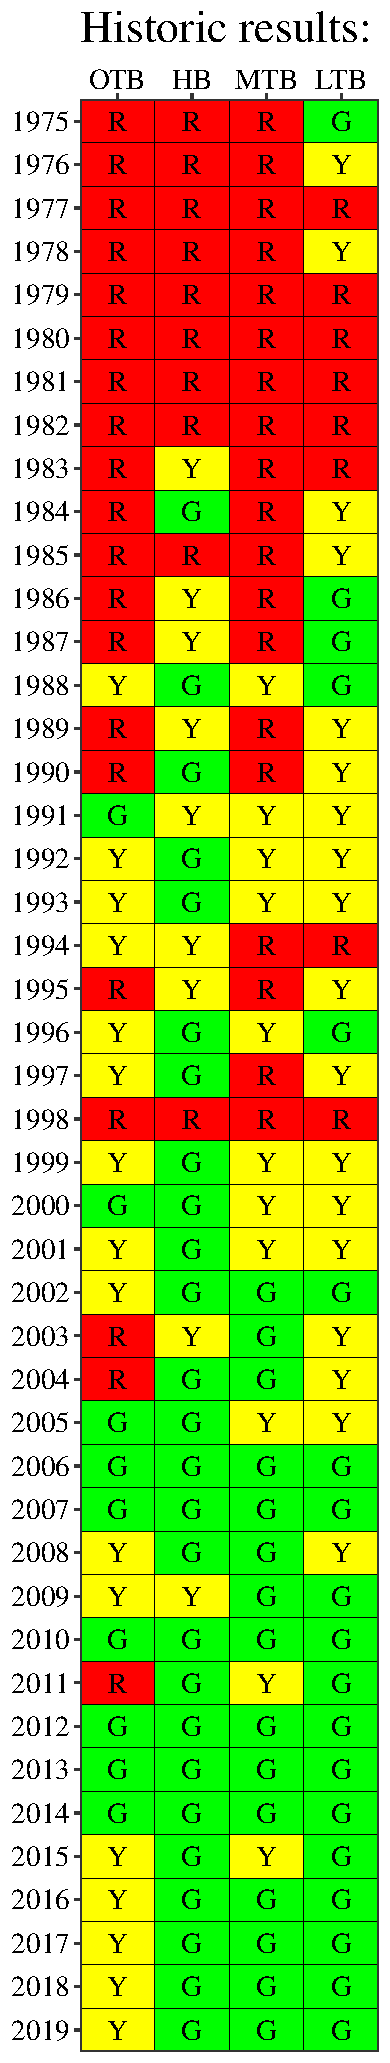
\includegraphics[trim = 0cm 0cm 0cm 0cm, width=1.1\linewidth]{figure/attainmat.pdf}}
\caption{\footnotesize Decision matrix results for 1975 to 2019.}
\label{fig:attainmat}
\end{figure}

\end{column}

%%%%%%%%%%%%%%
% right
%%%%%%%%%%%%%%    
\begin{column}{.65\linewidth}

\begin{block}{Background}
\begin{minipage}{0.5\textwidth}
\footnotesize
Light availability to seagrass is the guiding paradigm for TBEP's Nitrogen Management Strategy. Because excessive nitrogen loads to the bay generally lead to increased algae blooms (higher chlorophyll-a levels) (Figure 1) and reduce light penetration to seagrass, an evaluation method was developed to assess whether load reduction strategies are achieving desired water quality results (i.e. reduced chlorophyll-a concentrations and increased water clarity). 
\end{minipage}
\hspace{0.01in}
\begin{minipage}{0.45\textwidth}
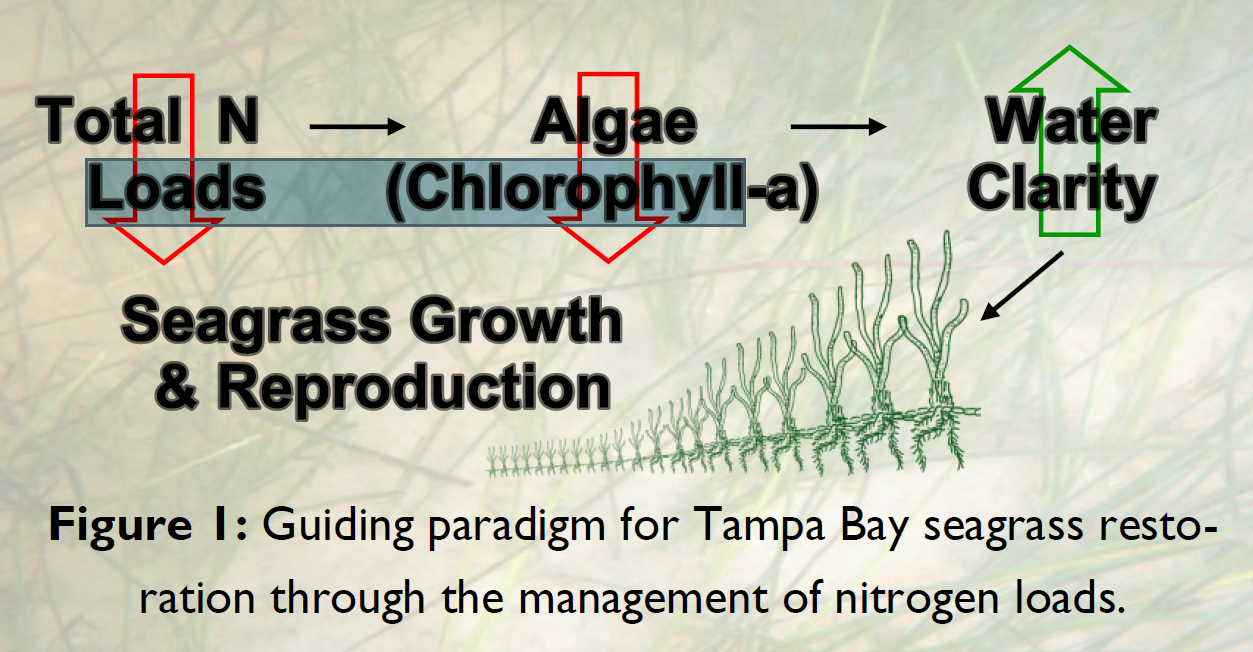
\includegraphics[width=\textwidth]{www/nitro.PNG}
\end{minipage}
\end{block}

\begin{block}{Decision Support Approach}
\begin{minipage}{0.5\textwidth}
\footnotesize
Year to year algae abundance (measured as chlorophyll-a concentrations) and visible light penetration through the water column (depth of secchi disk visibility) have been identified as critical water quality indicators in Tampa Bay. Tracking the attainment of bay segment specific targets for these indicators provides the framework for developing and initiating bay management actions. TBEP management actions adopted in response to the annually-assessed decision support results are shown to the right.
\end{minipage}
\hspace{0.01in}
\begin{minipage}{0.45\textwidth}
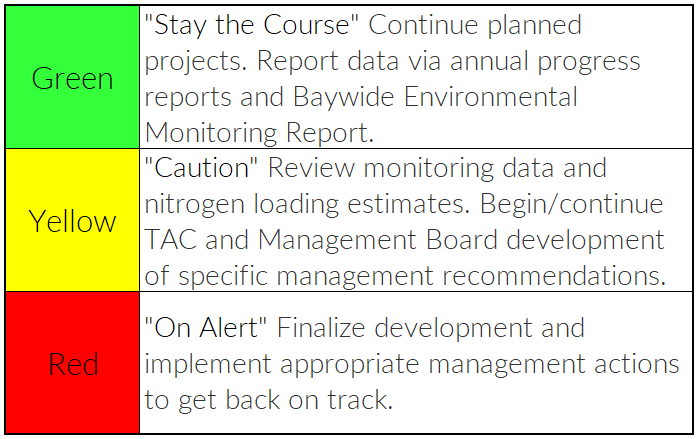
\includegraphics[width=\textwidth]{www/stoplight.PNG}
\end{minipage}
\end{block}

\begin{block}{2019 Decision Matrix Results}
\begin{minipage}{0.4\textwidth}
\footnotesize
Water quality (chlorophyll-a and light penetration) remained supportive of seagrass in Hillsborough Bay (HB), Middle Tampa Bay (MTB), and Lower Tampa Bay (LTB)(Table \ref{tab:segtab}, Figure \ref{fig:thrplot}). The nuisance alga, \textit{Pyrodinium bahamense}, was again reported in Old Tampa Bay (OTB) during the Summer and Fall 2019, contributing to a small magnitude chlorophyll-a exceedance. In all bay segments, separate algal bloom events contributed to individual stations exceeding the bay segment chlorophyll-a targets (Figure \ref{fig:sitemap}). However, effective light penetration was supportive of seagrass in all bay segments (Table \ref{tab:segtab}).
\end{minipage}
\hspace{0.01in}
\begin{minipage}{0.5\textwidth}
\footnotesize
%latex.default(tab, file = "", caption = cap.val, caption.loc = "top",     cgroup = cgrps, n.cgroup = c(2, 2, 1), rowlabel = "\\parbox{0.5cm}{Bay segment}",     colheads = c(maxyr, "target", maxyr, "target", "\\hspace{-0.3cm}\\parbox{0.7cm}{outcome}"),     label = "tab:segtab", col.just = rep("p{0.25in}", 6), table.env = F)%
\begin{table}[!tbp]
\caption{{\footnotesize Observed water quality indicators \& recommended management outcomes for 2019.}\label{tab:segtab}} 
\begin{center}
\begin{tabular}{lp{0.25in}p{0.25in}cp{0.25in}p{0.25in}cp{0.25in}}
\hline\hline
\multicolumn{1}{l}{\bfseries \parbox{0.5cm}{Bay segment}}&\multicolumn{2}{c}{\bfseries Chl-a (ug/L)}&\multicolumn{1}{c}{\bfseries }&\multicolumn{2}{c}{\bfseries \parbox{1.5cm}{Effective Light Penetration ($m^{-1}$)}}&\multicolumn{1}{c}{\bfseries }&\multicolumn{1}{c}{\bfseries }\tabularnewline
\cline{2-3} \cline{5-6}
\multicolumn{1}{l}{}&\multicolumn{1}{c}{2019}&\multicolumn{1}{c}{target}&\multicolumn{1}{c}{}&\multicolumn{1}{c}{2019}&\multicolumn{1}{c}{target}&\multicolumn{1}{c}{}&\multicolumn{1}{c}{\hspace{-0.3cm}\parbox{0.7cm}{outcome}}\tabularnewline
\hline
OTB&$10.64$&$ 8.5$&&$0.76$&$0.83$&&\cellcolor{yellow}yellow\tabularnewline
HB&$11.31$&$13.2$&&$0.97$&$1.58$&&\cellcolor{green}green\tabularnewline
MTB&$ 5.83$&$ 7.4$&&$0.59$&$0.83$&&\cellcolor{green}green\tabularnewline
LTB&$ 4.05$&$ 4.6$&&$0.61$&$0.63$&&\cellcolor{green}green\tabularnewline
\hline
\end{tabular}\end{center}
\end{table}

\end{minipage}

\end{block}

\vspace{-0.2in}

\begin{columns}[t]



\begin{column}{0.67\textwidth}
\vspace{-0.47cm}
\begin{figure}[htbp]
% \hspace*{2cm} 
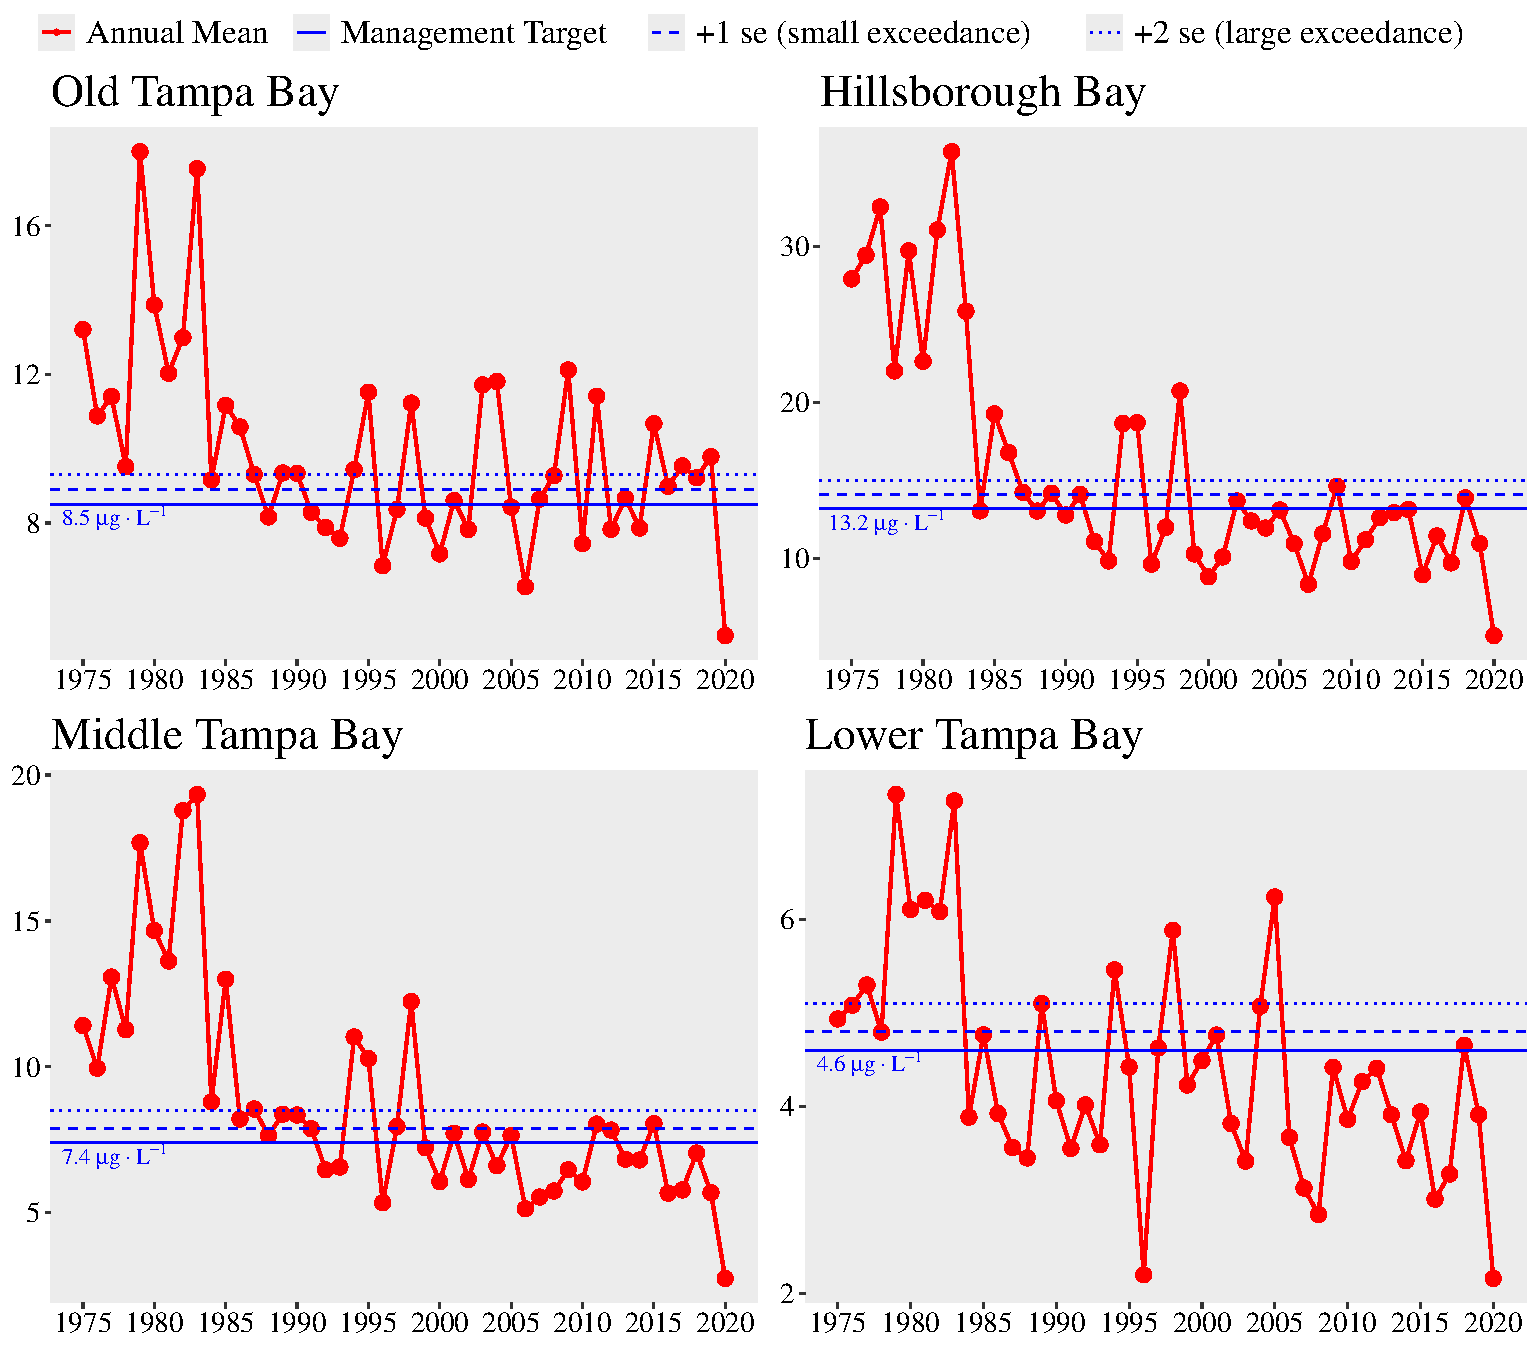
\includegraphics[trim = 0cm 0cm 0cm 0cm, width=1.1\linewidth]{figure/thrplot.pdf}
\caption{\footnotesize Historic chlorophyll-a annual averages for the four bay segments.}
\label{fig:thrplot}
\end{figure}

\end{column}



